\section{Hash de contraseñas: Bcrypt}\label{secc:bcrypt}

Bcrypt es un algoritmo de hash que apunta a ser lento
\autocite{stackexchange-bcrypt}.
El algoritmo deriva del codificador de bloques simétricos Blowfish, y es lento
por diseño, ya que su uso es proteger contraseñas, y hace así más difícil un
ataque de diccionario \autocite{auth0-bcrypt}.

Se considera el estándar \emph{defacto} para el almacenamiento de contraseñas
\autocite{itblog-pwhash}, dada una de sus características: el poder adaptarse
al nuevo hardware (más rápido) haciéndose aún más lento con el ajuste de un
parámetro \autocite{auth0-bcrypt}. 
Otra ventaja es que incluye por defecto el uso de \emph{salting}
\autocite{stackexchange-bcryptsalt} y evita así ataques de \emph{rainbow
table}.
Este valor se almacena codificado en el valor resultante lo que permite
verificar mas adelante una contraseña repitiendo el proceso con el mismo
valor para salt.

\section{Derivación de Claves: Argon2}\label{secc:argon}

El algoritmo recomendado por la ``Password Hashing Competition'' \autocite{phc},
que evalúa algoritmos con un proceso similar a NIST en sus competencias AES y
SHA-3.
Es el algoritmo elegido por KeePass, un administrador de contraseñas de código
libre, para derivar una clave y cifrar los datos \autocite{keepass}.

Utiliza un salt (\autoref{secc:bcrypt}) para calcular sus hashes.
Este hash lo generamos al igual que el token (\autoref{secc:token}),
un vector de 16 bytes (128 bits, que es el defecto de la librería) con valores
aleatorios.

Para generar una clave usamos los siguientes parámetros:
\begin{itemize}
	\item 5 iteraciones
	\item 65536 kibibytes de memoria utilizados
	\item 1 solo hilo para calcularlo
\end{itemize}

Los valores de estos parámetros son los básicos recomendados por la 
documentación.~\cite{argon2-jvm}
Al llevar esta aplicación a su hardware de servidor final de deben ajustar estos
parámetros, ya que la idea es que sean tan altos como sea posible antes de que
afecten negativamente la experiencia del usuario (ya que tomarán mas tiempo).

Este es un beneficio de Argon2 (al igual que de Bcrypt) ya que pueden ajustar
su ``costo'' e \emph{ineficiencia} a medida que mejora el hardware haciendo más 
difíciles los ataques de fuerza bruta.

Almacenamos el valor de salt en la base de datos, tabla \code{Usuario}, para
poder más adelante repetir el proceso, y obtener la misma clave derivada.


\section{Cifrado simétrico de archivos}

\subsection{AES}\label{secc:aes}

El algoritmo AES es el algoritmo de elección para la mayoría de aplicaciones 
modernas que busquen proteger datos o archivos \autocite{cryptomathic-aes}.

El cifrado tiene una longitud variable de bloque y de clave, con
especificaciones para claves con una longitud de 128, 192 o 256 bits para cifrar 
bloques con una longitud de 128, 192 o 256 bits. Tanto la longitud del bloque 
como la longitud de la clave se pueden extender por 
múltiplos de 32 bits \cite{coulouris}.

Aunque una clave mayor hace más difícil que esta se descubra también hace más
lento el proceso, por lo que se debe pesar el valor riesgo contra el impacto
en uso de recursos para decidir qué algoritmo usar.
AES con claves de 256 bits, por ejemplo, es un 40\% más lento que su uso con claves
de 192 bits \autocite{solarwinds-aes}.
Considerando sin embargo que nuestra aplicación busca proteger los datos de los
usuarios durante su intercambio elegimos AES-256.

\subsection{Blowfish}\label{secc:blowfish}

Este algoritmo tiene un tamaño de bloque de 64 bits y un tamaño de clave que 
varía de 32 a 448 bits y se optimizó para CPU de 32 bits. Puede ser usado como 
reemplazo para DES o IDEA \cite{schneier}

Al día de hoy se considera un algoritmo de cifrado seguro, aunque al usar un 
bloque de 64 bits es vulnerable a un tipo específico de ataque criptográfico 
de fuerza bruta conocido como \emph{birthday attack} \cite{geeksBlowfish}.

\subsection{TEA}\label{secc:tea}

Este algoritmo está programado en C y utiliza un bloque de 64 bits representado 
por dos enteros de 32 bits en el vector llamado \emph{text[]}. 
La clave es de 128 bits, representada por cuatro enteros de 32 bits. 
TEA es tiene la capacidad de proveer un encriptado de clave secreta 
razonablemente rápido y seguro. Se destaca por ser un programa muy consiso, lo 
favorece la optimización y la implementación por hardware.
También se conoce que es más rápido que el algorítmo DES \cite{coulouris}.
%TODO: Es seguro hoy en dia?
Una desventaja es que este algoritmo es vulnerable a los ataques de claves 
relacionadas. Esto no es un problema cuando la clave es aleatoria, pero tampoco 
inspira confianza, ya que esta vulnerabilidad y la posiblidad de la existencia de 
claves equivalentes triviales no fueron consideradas en el artículo original 
\cite{stackexchange-crypto-tea}.

Este algoritmo generalmente es seguro cuando se cumplen las siguientes 
condiciones: 
las claves son aleatorias (el cambio de clave debe ser atómico y con una nueva 
clave aleatoria); el tamaño del bloque de 64 bits no es una preocupación,
(por ejemplo, se usa un modo de operación diferente al ECB y la clave se cambia 
antes de un valor de 1GB de datos); la relativa lentitud no es un obstáculo; 
los ataques de canales laterales no son un problema \cite{stackexchange-crypto-tea}.

%https://crypto.stackexchange.com/questions/16186/is-tea-considered-secure

\subsection{DES y 3DES}\label{secc:DES}

Su función de encriptado mapea una entrada de texto plano de 64 bits a una 
salida encriptada de 64 bits, utilizando una clave de 56 bits \cite{coulouris}.
En 1997 se demostró que este algorítmo es vulnerable a ataques de fuerza bruta 
mediante un ataque exitoso de ese tipo y por lo tanto debe ser considerado 
obsoleto para la protección de cualquier tipo de información, con excepción de 
aquella que sea de poco valor \cite{coulouris}.

Una alternativa es utilizar \emph{3DES (triple-DES)} que consiste en aplicar DES 
tres veces y con dos claves, K\textsubscript{1} y K\textsubscript{2}:

\[E\textsubscript{3DES}(K\textsubscript{1}, K\textsubscript{2}, M) = 
E\textsubscript{DES}(K\textsubscript{1}, D\textsubscript{DES}
(K\textsubscript{2}, E\textsubscript{DES}(K\textsubscript{1}, M)))\]

Esto le da una robustéz contra los ataques de fuerza bruta equivalente a la que 
se tiene cuando se usa una clave de 112 bits pero tiene la desventaja de tener 
mal rendimiento, que resulta de la aplicación triple de un algoritmo que ya es 
lento de por sí según estándares modernos \cite{coulouris}.

\begin{figure}[H]
    \centering
        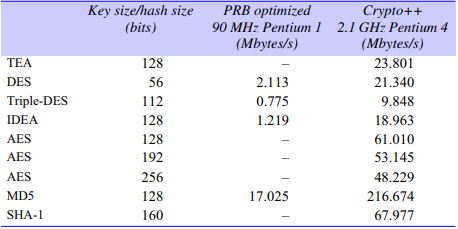
\includegraphics{img/rendimientoAlgoritmos.PNG}
    \caption{Rendimiento de algoritmos de cifrado simétrico y 
    \emph{secure digest} \cite{coulouris}.}
    \label{tabla:rendimiento}
\end{figure}


% TODO: source https://www.bsi.bund.de/SharedDocs/Downloads/EN/BSI/Publications/TechGuidelines/TG02102/BSI-TR-02102-1.pdf;jsessionid=139E7E1917DFDEAF23598BDC2CE60B01.1_cid341?__blob=publicationFile&v=9

\section{Cifrado Asimétrico}

\subsection{RSA}\label{secc:rsa}

Este algoritmo se basa en el uso del producto de dos números primos que son 
\(> 10^{100}\), respaldandose en el hecho de que la determinación de los factores 
primos de números tan grandes es un proceso muy costoso a nivel computacional y 
tomaría una gran cantidad de tiempo, aún en computadoras de alto rendimiento. 
El producto de dos números que son  \(> 10^{100}\) es  
\(> 10^{200}\) y la factorización de dicho número, según un cálculo realizado 
en 2012, puede demorar alrededor de un millon de años. 
A pesar de que se han realizado extensas investigaciones, no se le encontraron 
fallas y es ampliamente utilizado hoy en día \cite{coulouris}.

Vale la pena señalar una debilidad potencial de todos los algoritmos de clave 
pública es que, como la clave pública está disponible para los atacantes, estos pueden 
generar fácilmente mensajes cifrados.
Por lo tanto, pueden intentar descifrar un mensaje desconocido cifrando exhaustivamente
secuencias de bits arbitrarias hasta que se logra una coincidencia con el mensaje 
de destino. Este ataque que se conoce como un \emph{chosen plaintext attack}, se 
vence asegurando que todos los mensajes
sean más largos que la longitud de la clave, por lo que esta forma de ataque de 
fuerza bruta es menos factible que un ataque directo a la llave \cite{coulouris}.

RSA y otras formas de criptografía asimétrica que usan la multiplicación de 
números primos como su \emph{one-way function} serán vulnerables si se descubre 
un algoritmo de factorización más rápido \cite{coulouris}.

\subsection{Algoritmos de curvas elípticas}\label{secc:elliptic}

Estos algoritmos generan los pares de claves pública/privada basandose en las 
propiedades de las curvas 
elípticas. A diferencia de RSA, su seguridad no depende de la dificultad de 
factorizar números grandes.
Las principales ventajas que ofecen sobre RSA son que los requerimientos de 
procesamiento para el cifrado y el descifrado son menores y que claves 
más pequeñas también son seguras \cite{coulouris}.

Lamentablemente no existen muchas API's disponibles que implementen este tipo de 
algoritmos, y se mantengan actualizadas. La más utilizada parece ser una 
llamada \emph{Bouncy Castle Crypto API} que funciona con Java y C\#, 
y presenta el paquete org.bouncycastle.crypto.ec que contiene implementaciones 
para una variedad de transformaciones criptográficas de curvas elípticas como 
\emph{EC ElGamal} \cite{bouncycastle}.

\section{Protocolos criptográficos híbridos}\label{secc:hybrid}
Dado que los algoritmos de cifrado simétrico son significativamente más rápidos 
que los asimétricos, 
si se intenta cifrar un archivo pesado con cifrado asimétrico, el proceso de 
cifrado y descifrado va a requerir demasiado tiempo. 
En cambio, si se encripta solo la clave simétrica mediante cifrado asimétrico 
y luego se utiliza la clave simétrica para cifrar y descifrar el archivo 
pesado, el proceso de encripción será más rápido y eficiente. 
\cite{stackexchange-hybrid}.

Este tipo de combinación también permite cifrar el mensaje eficientemente para 
múltiples destinatarios. Si solamente se utilizara el cifrado asimétrico, se 
tendría que cifrar todo 
el mensaje varias veces, una vez para cada destinatario. Pero con el cifrado 
híbrido solo se necesita cifrar varias copias de la clave simétrica y una 
copia del mensaje \cite{stackexchange-hybrid}.

% TODO: Lo comento porque en no hacemos esto, y quedamos en offside 😆
% Otra ventaja del cifrado híbrido es que nunca envía el mismo texto cifrado dos 
% veces. Se genera, o se debe generar, una nueva clave simétrica para cada mensaje. 
% Esto significa que cuando el mismo texto plano se cifra dos veces para un  
% mismo receptor, los cifrados se verán diferentes. Mientras que si se utilizara 
% únicamente la clave pública, ambos cifrados serían idénticos \cite{stackexchange-hybrid}.

Debido a las ventajas que presenta un protocolo híbrido, el sistema desarrollado 
(\autoref{secc:esquemacifrado}) implementa un protocolo 
criptográfico híbrido en el que se utiliza RSA para el cifrado asimétrico 
\autocite{ppt202}, con claves de 2048 bits y AES-256 para el simétrico. 
Más adelante se justifica la elección de los algoritmos.

\section{Justificación de los algoritmos elegidos}

Con la finalidad de proteger el sistema de la mejor manera se elige 
utlizar un sistema híbrido con los siguentes algoritmos.

Para el cifrado simétrico se elige utilizar AES-256 CBC por varias razones. 
La princial es que, como la NSA 
considera que la utilización de este algoritmo con ese largo de clave es 
suficiente para proteger información clasificada de todos los 
niveles, hasta TOP SECRET, consideramos que tiene excelentes referencias y que 
es más que suficiente para proteger nuestro sistema. También por la alta 
disponibilidad de librerías confiables y actualizadas que permiten una 
implementación segura y robusta del algoritmo. De los algoritmos disponibles es 
de los que ofrece mejor rendimiento (\autoref{tabla:rendimiento}) y seguridad, 
ya que en aproximadamente 19 años desde su publicación no se conocen ataques 
que afecten gravemente la seguridad del algoritmo. 

Si bien existen ataques de 
canal lateral contra algunas implementaciones de AES, no existen ataques 
criptoanalíticos prácticos contra el algoritmo abstracto. 
El mejor ataque criptoanalítico contra el cifrado completo en un modelo de 
ataque razonable es probablemente el ataque \emph{biclique}, que quita como máximo 4 
bits de la clave.
En el caso de que se quitaran 4 bits de la clave, quedarían todavia 252 bits. 
Dicho de otra manera, para llevar a cabo estos ataques se necesitaría gastar un esfuerzo 
aproximadamente proporcional a un ataque de fuerza bruta forzando una clave AES 
donde ya conocían cuatro bits de la clave y esto tomaría aproximadamente \(2^{252}\)
operaciones, manteniendo un margen de seguridad más que suficiente 
\cite{stackexchange-crypto-biclique}.

Para el cifrado asimétrico se elige RSA con claves de 2048 bits que es el largo 
de clave recomendado por NIST \cite{NIST-RSA}. En cuanto a los ataques posibles 
contra este algoritmo, si bien se han realizado una cantidad de ataques, 
ninguno de estos es devastador.

Se elige este tipo de algoritmo por sobre los de curvas elípticas porque hay  
una mayor cantidad de librerias disponibles que lo implementan de manera segura 
y que han sido probadas exhaustivamente.
